% \iffalse
\let\negmedspace\undefined
\let\negthickspace\undefined
\documentclass[journal,12pt,twocolumn]{IEEEtran}
\usepackage{cite}
\usepackage{amsmath,amssymb,amsfonts,amsthm}
\usepackage{algorithmic}
\usepackage{graphicx}
\usepackage{textcomp}
\usepackage{xcolor}
\usepackage{txfonts}
\usepackage{listings}
\usepackage{enumitem}
\usepackage{mathtools}
\usepackage{gensymb}
\usepackage{comment}
\usepackage[breaklinks=true]{hyperref}
\usepackage{tkz-euclide} 
\usepackage{listings}
\usepackage{gvv}                                        
\def\inputGnumericTable{}                                 
\usepackage[latin1]{inputenc}                                
\usepackage{color}                                            
\usepackage{array}                                            
\usepackage{longtable}                                       
\usepackage{calc}                                             
\usepackage{multirow}                                         
\usepackage{hhline}                                           
\usepackage{ifthen}                                           
\usepackage{lscape}

\newtheorem{theorem}{Theorem}[section]
\newtheorem{problem}{Problem}
\newtheorem{proposition}{Proposition}[section]
\newtheorem{lemma}{Lemma}[section]
\newtheorem{corollary}[theorem]{Corollary}
\newtheorem{example}{Example}[section]
\newtheorem{definition}[problem]{Definition}
\newcommand{\BEQA}{\begin{eqnarray}}
\newcommand{\EEQA}{\end{eqnarray}}
\newcommand{\define}{\stackrel{\triangle}{=}}
\theoremstyle{remark}
\newtheorem{rem}{Remark}
\begin{document}
\parindent 0px

\bibliographystyle{IEEEtran}
\vspace{3cm}

\title{Assignment\\[1ex]GATE-EE-50}
\author{EE23BTECH11034 - Prabhat Kukunuri$^{}$% <-this % stops a space
}
\maketitle
\newpage
\bigskip

\renewcommand{\thefigure}{\theenumi}
\renewcommand{\thetable}{\theenumi}
\section{Question}
The discrete-time Fourier transform of a signal x\sbrak{n} is $X\brak{\Omega}=\brak{1+\cos{\Omega}}e^{-j\Omega}$. Consider that $x_{p}\sbrak{n}$ is a periodic signal of period $N=5$ such that
\begin{align}
    x_p\sbrak{n}&=x[n],\text{for n= 0, 1, 2}\\
    &=0,\text{for n= 3, 4}
\end{align}
Note that $x_p\sbrak{n}=\sum_{k=0}^{N-1}a_{k}e^{j\frac{2\pi}{N}kn}$. The magnitude of the Fourier series coefficient $a_3$ is \rule{3cm}{0.15mm} \brak{\text{Round off to 3 decimal places}}.\\
\solution\\
\begin{table}[h!]
    \centering
    \begin{tabular}{|p{2cm}|p{2.80cm}|p{2.70cm}|}
    \hline
    Symbol&Value&Description\\ \hline
    $$x(n)$$&$$(x(0)+nd)u(n)$$&$$n^{th}$$ term of an A.P\\ \hline
    $$x(0)$$&$$x(0)$$&$1^{st}$ term of the A.P\\ \hline
    $$d$$&$$d$$&Common difference\\ \hline
    $$y(n)$$&$$x(n)\ast u(n)$$&Sum of n terms of an AP\\ \hline
    $$a$$&$$y(p-1)$$&Sum of first p terms of the AP\\ \hline
    $$b$$&$$y(q-1)$$&Sum of first q terms of the AP\\ \hline
    $$c$$&$$y(r-1)$$&Sum of first r terms of the AP\\ \hline
\end{tabular}
    \caption{variable description}
    \label{tab:my_label}
\end{table}\\
Using Euler's form of representation of complex numbers,
\begin{align}
    e^{j\Omega}=\cos{\Omega}+j\sin{\Omega}
\end{align}
$X\brak{\Omega}$ can be expressed as,
\begin{align}
    X\brak{\Omega}=\frac{1}{2}+e^{-j\Omega}+\frac{e^{-j2\Omega}}{2}
\end{align}
As sampling frequency is $1Hz$ \brak{\omega=\Omega} from DTFT(discrete time fourier transform) we get,
\begin{align}
    X\brak{\Omega}&=\sum^{n=2}_{n=0}x\brak{n}e^{-j\omega n},   \omega \in \brak{-\pi,\pi}\\
    X\brak{\Omega}&=\frac{1}{2}+e^{-j\Omega}+\frac{e^{-j2\Omega}}{2}
\end{align}
On comparing coefficients we get,
\begin{align}
    x\brak{n}&=
    \begin{cases}
        \dfrac{1}{2} & \text{if n=0}\\
        1 & \text{if n=1}\\
        \dfrac{1}{2} & \text{if n=2}\\
        0 & \text{if n$\neq$\cbrak{0,1,2} }
    \end{cases}\\
    x_{p}\brak{n}&=\sbrak{\frac{1}{2},1,\frac{1}{2},0,0} \text{with period, N=5}\\
    a_3&=\frac{1}{5}\sum^{4}_{n=0}x\brak{n}e^{-\frac{j6\pi}{5}n}\\
    |a_3|&=0.038
\end{align}
\begin{figure}[ht]
    \centering
    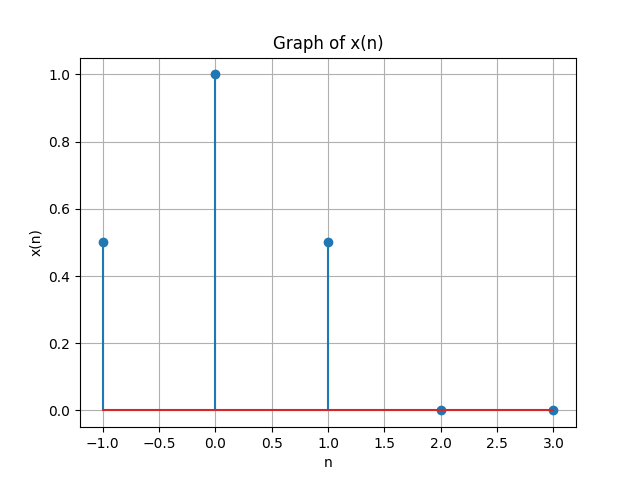
\includegraphics[width=\columnwidth]{figs/Figure_1.png}
    \caption{Plot of x(n) $vs$ n}
    \label{fig:50.1}
\end{figure}
\begin{figure}[ht]
    \centering
    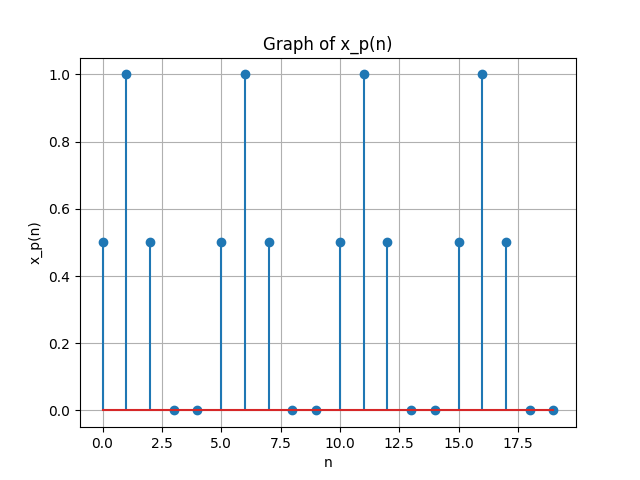
\includegraphics[width=\columnwidth]{figs/Figure_2.png}
    \caption{Plot of $x_p(n)$ $vs$ n}
    \label{fig:50.2}
\end{figure}
\begin{figure}[ht]
    \centering
    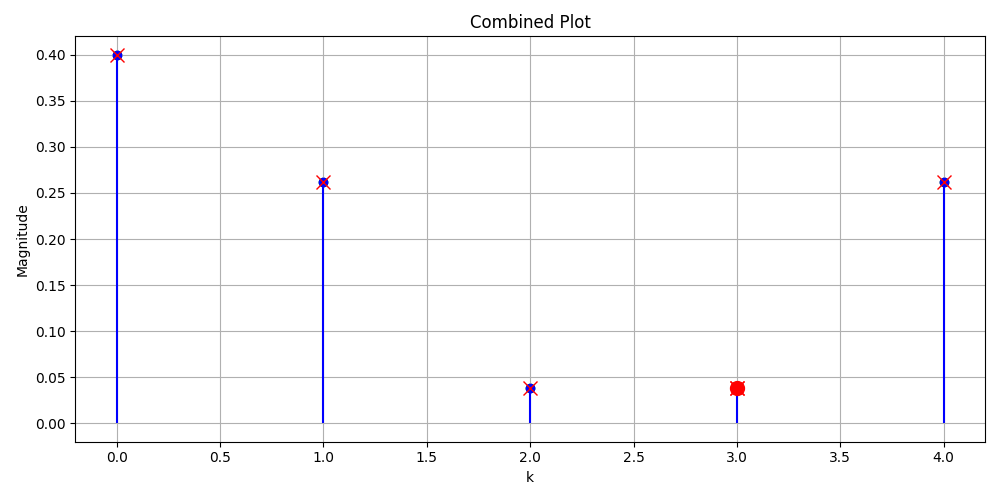
\includegraphics[width=\columnwidth]{figs/Figure_3.png}
    \caption{Plot of $x_p(n)$ $vs$ n}
    \label{fig:50.3}
\end{figure}
\end{document}
